\section{RESULTS}
\subsection{RQ1. Barriers as Asymmetries in Accessible Video Creation Education}

We synthesize the observed barriers across both in-person ([City 1]) and online ([City 2]) workshops as three interlocking asymmetries: expertise, tools and ecosystems, and interaction paradigms. These asymmetries manifested differently across delivery modes but consistently shaped collaboration across tutor–participant, participant–helper, participant–participant, and tutor–helper relationships. In this section, helpers refer to support workers who accompanied some participants. 

\subsubsection{Expertise asymmetry: video pedagogy vs access pedagogy}

While all tutors possessed strong video production expertise, translating this knowledge into accessible instruction revealed fundamental gaps between visual and non-visual pedagogical approaches. The workshops exposed three critical areas where traditional video pedagogy failed to bridge the accessibility divide.

\textbf{Translation gap between visual and non-visual mental models. }
Tutors who understood timeline editing struggled to convey it non-visually. P3 ([City 2]) remarked, “Some of the words you’re using here, like position the playhead... I’ve got absolutely no idea about the wording.” In [City 1] Workshop 1, a low-vision tutor attempted to guide a blind participant out of the recording feature: “do up swipe like, up and down. And then you can click on the red button, and it will start.” The mixed instruction (gesture plus a colour-based visual referent) illustrates how visual framing persisted even when non-visual navigation was required.

\textbf{Tutor–sighted-guide coordination gap.} Helpers were not part of formal instruction, but they inevitably took on assistance tasks (for example, device positioning, noting steps, reading out menu states). Their effectiveness varied by digital competence and familiarity with the participant. Some pairs coordinated smoothly and provided more support; others contributed little beyond basic prompts. Since helpers received no role briefing or VoiceOver orientation, support quality remained uneven across participants.

\textbf{Documentation and retention gap.} The absence of accessible, stepwise artifacts (e.g., text/audio checklists aligned to VoiceOver and magnifier workflows) shifted learning into short-term memory. As P4 ([City 2]) put it, “I couldn’t find any way for writing them down… it became a memory exercise.” This amplified the pacing asymmetry: without persistent materials, participants could not review or practice between sessions, and tutors had to re-teach procedures in subsequent meetings.
(Following participant feedback from the first workshop, we developed accessible workbooks with step-by-step instructions broken down into granular VoiceOver-compatible steps. This documentation, combined with session slides and audio recordings, significantly improved retention and between-session practice.)

\subsubsection{Tool and Ecosystem Asymmetry: Platform Fragmentation }

\textbf{Application-accessibility incompatibility.} Core editing applications (CapCut, Videoleap) were non-functional with screen readers, blocking blind participants despite their motivation and effort. 

\textbf{Operating system divisions.} The iOS-centric curriculum reduced engagement for Android users. In [City 1], two Android participants could not follow iOS-specific segments. Online, requests for Android coverage (for example, Open Camera) received limited follow-through. Even within iOS, device variations created confusion, for example participants noted iMovie on iPad had more hierarchical menus than on iPhone.

\textbf{Workflow-level friction rather than app-level absolutes.} Rather than a single app being strictly unusable, participants encountered practical breakdowns when screen reader navigation and editor workflows did not align in-session, which led to abandoned steps and detours. During [City 1] Workshop 2, P6 attempted to trim a video clip in iMovie. The participant could navigate to the timeline using VoiceOver, which announced "timeline, adjustable" when reached. However, determining the playhead's exact position required visual feedback that VoiceOver couldn't provide.
(80\% of our participants, sustainability, limitation, )

\subsubsection{Interaction paradigm asymmetry: Competing Navigation Models}
Fundamental differences between visual touch and screen reader gesture models created persistent collaboration barriers.

\textbf{Dual instruction burden. }Each technique required parallel explanation across paradigms. Low-vision participants could follow “press the red button,” while blind participants needed instructions grounded in element order and audio labels. Attempting both tracks simultaneously slowed progress and introduced confusion. Online, this surfaced as focus-control difficulties, for example P4 ([City 2]) noted, “with my four-minute video, it’s just whizzing through it a bit.”

\textbf{Cognitive load from paradigm switching.} Translating each step across visual–spatial references (“press the red button”) and non-visual traversal (element order + labels via VoiceOver) demanded continuous remapping by blind participants,and by tutors narrating both tracks. In noisy rooms, earphone use to hear VoiceOver improved access but further limited overheard feedback and ad-hoc assistance, compounding cognitive effort.

\textbf{Helper–participant navigation disconnect. }With screen curtain enabled, displays were not visible by design, eliminating visual guidance routes for helpers. Even with screen curtain off, helpers’ mental models did not match VoiceOver’s gesture grammar, limiting them to minimal prompts such as “next one,” “confirm,” and “go back.” In louder in-person rooms, several screen reader users used earphones to hear VoiceOver. This improved their own access but further limited the possibility of ad hoc support from tutors or nearby peers who could not hear the screen reader feedback.

\textbf{Group-level access conflicts. }Mixed-ability groups faced competing needs that could not be simultaneously met. Magnifier-optimized instructions confused screen reader users, while detailed verbal descriptions for blind participants slowed those with residual vision. Participants recognized this tension: "It's always difficult when you've got a mixture of totally blind and partials... trying to adjust to the different needs." The feedback to create "two different groups... one only screen readers, one uses magnifiers" acknowledged these fundamental incompatibilities.

\subsubsection{Delivery Mode Trade-offs: Co-located vs Remote }
\textbf{Co-located affordances and constraints.} In-person sessions enabled tactile and embodied learning with cameras, rigs, and phones. Participants could “touch it and use it,” and tutors could adjust posture, framing, or grip. These benefits required intensive individualized facilitation that was difficult to scale in moments of divergence across access modalities.

 \textbf{Remote affordances and constraints.} Online sessions supported replay and self-pacing but limited physical device demonstration. Certain concepts, for example stabilization or tripod setup, were hard to convey without hands-on interaction. File transfer remained a recurring barrier, with cloud storage failing unpredictably for some participants and preventing cross-device sharing at critical moments.

\subsection{RQ2. Collaborative patterns emerge in ability-diverse video creation education }

Our analysis reveals that different combinations of vision abilities produce distinct collaborative strategies and interaction patterns. Rather than viewing visual impairment as an individual attribute, we found that collaborative dynamics emerged from the specific configurations of abilities within dyads and triads. Following our analytical approach, we identified four primary patterns, each with characteristic interactions, temporal organizations, and collaborative strategies that fundamentally shaped learning experiences in ability-diverse workshops.

 \begin{figure}
     \centering
     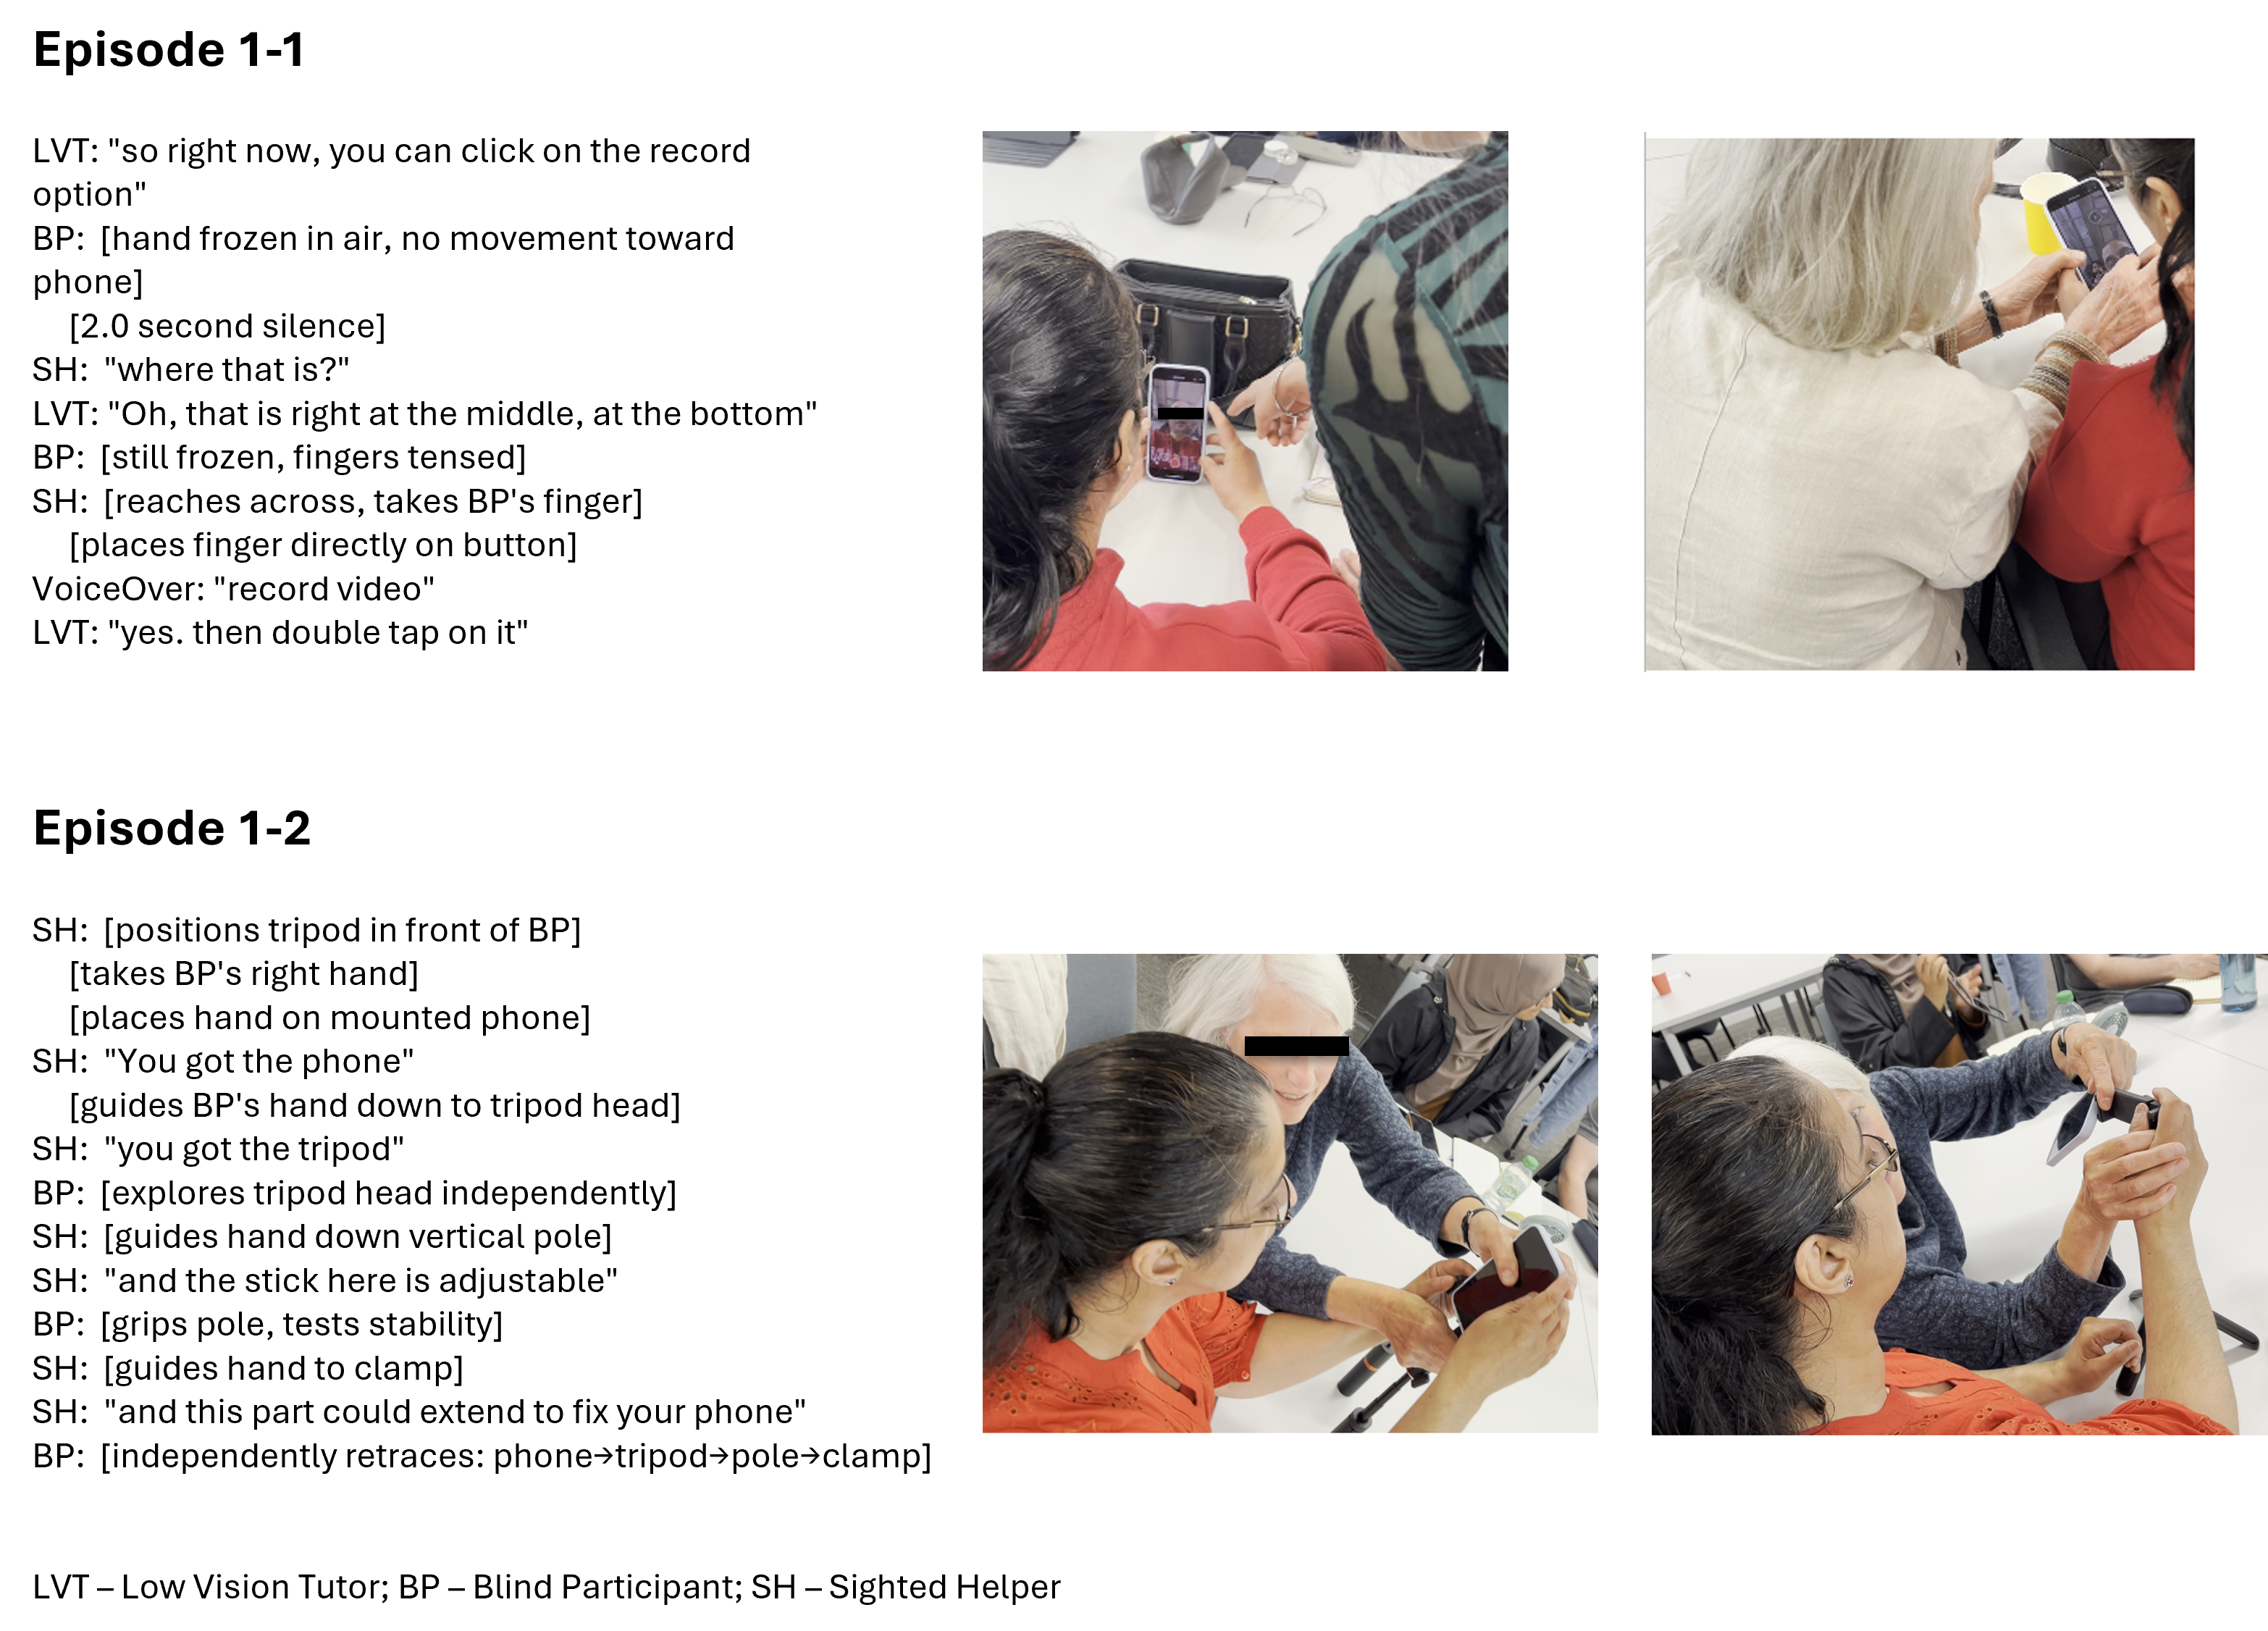
\includegraphics[width=1\linewidth]{Pics/Pattern_1.png}
     \caption{Collaborative patterns: : Direct haptic mediation (Episode 1 \& Episode 1-2)}
     \label{fig:paatern1}

\Description{Four-photo collage from a hands-on mobile-video workshop. Top left: a participant records a short clip of an older woman using a smartphone while others observe. Top right: an older woman guides two participants as they look at a phone together. Bottom left: two participants position a phone in a small clamp and discuss settings. Bottom right: participants fasten a phone onto a wrist-mount for wearable recording. The scenes emphasise peer instruction and shared manipulation of devices. }
 \end{figure}

\subsubsection{Pattern 1: Direct Haptic Mediation }
When blind and sighted (or partially sighted) participants collaborated, interactions consistently followed a pattern of direct haptic mediation, systematically bypassing verbal description in favour of physical guidance.

\textbf{Episode 1-1: Physical Placement Over Verbal Direction. }In the recording button episode from the [City 1] workshop ( \autoref{fig:paatern1}), we observe how verbal spatial descriptions fail to provide actionable information for blind participants, leading to immediate haptic intervention. The interaction begins with what appears to be a straightforward instruction from a low vision tutor: "so right now, you can click on the record option." However, this instruction lacks any spatial reference that would enable the blind participant to locate the button. The participant's response,hand frozen in air with no movement toward the phone,materially demonstrates complete spatial disorientation. The 2.0-second silence that follows is not merely a pause but what conversation analysts term a "dispreferred response" marker, indicating trouble in the interaction.

A sighted helper sitting beside the participant recognizes this trouble and intervenes with the critical question: "where that is?" This question does more than request information; it explicitly identifies the missing element in the tutor's instruction. The tutor's response:” Oh, that is right at the middle, at the bottom" provides visual-spatial coordinates that would be immediately actionable for a sighted person. 

However, the blind participant's continued frozen posture and tensed fingers reveal that these visual coordinates remain non-actionable. The visual-spatial framework of "middle" and "bottom" requires a mental model of the screen as a two-dimensional plane with established directional orientational, model that depends on visual access for its construction and maintenance. As Figure 1 shows, the sighted helper's immediate response represents a complete bypass of verbal-spatial description through direct finger placement on the button, followed by successful VoiceOver confirmation and the participant's independent double-tap execution. 

\textbf{Episode 1-2: Systematic Tactile Mapping. }For physical equipment introduction, blind-sighted dyads developed highly structured exploration patterns that revealed sophisticated understanding of non-visual spatial learning. In the tripod familiarization sequence (\autoref{fig:paatern1}), the sighted helper employed a methodical approach that systematically constructed a mental map through guided touch. The helper began by positioning the tripod directly in front of the blind participant, then took their right hand and placed it on the phone already mounted, providing the verbal anchor "You got the phone."

The exploration continued systematically downward,from phone to tripod head to vertical pole,with each component verbally labelled as the participant's hand made contact. Notably, between each guided segment, the blind participant engaged in independent exploration: fingers examining the tripod head's texture and joints, hands gripping the pole to test stability, and rotating the adjustment ring experimentally. These moments of autonomous investigation, interspersed between guided movements, demonstrate active learning rather than passive reception. The sequence concluded with the participant independently retracing the entire path from phone to clamp, confirming successful spatial map construction through haptic channels.
 \begin{figure}
     \centering
     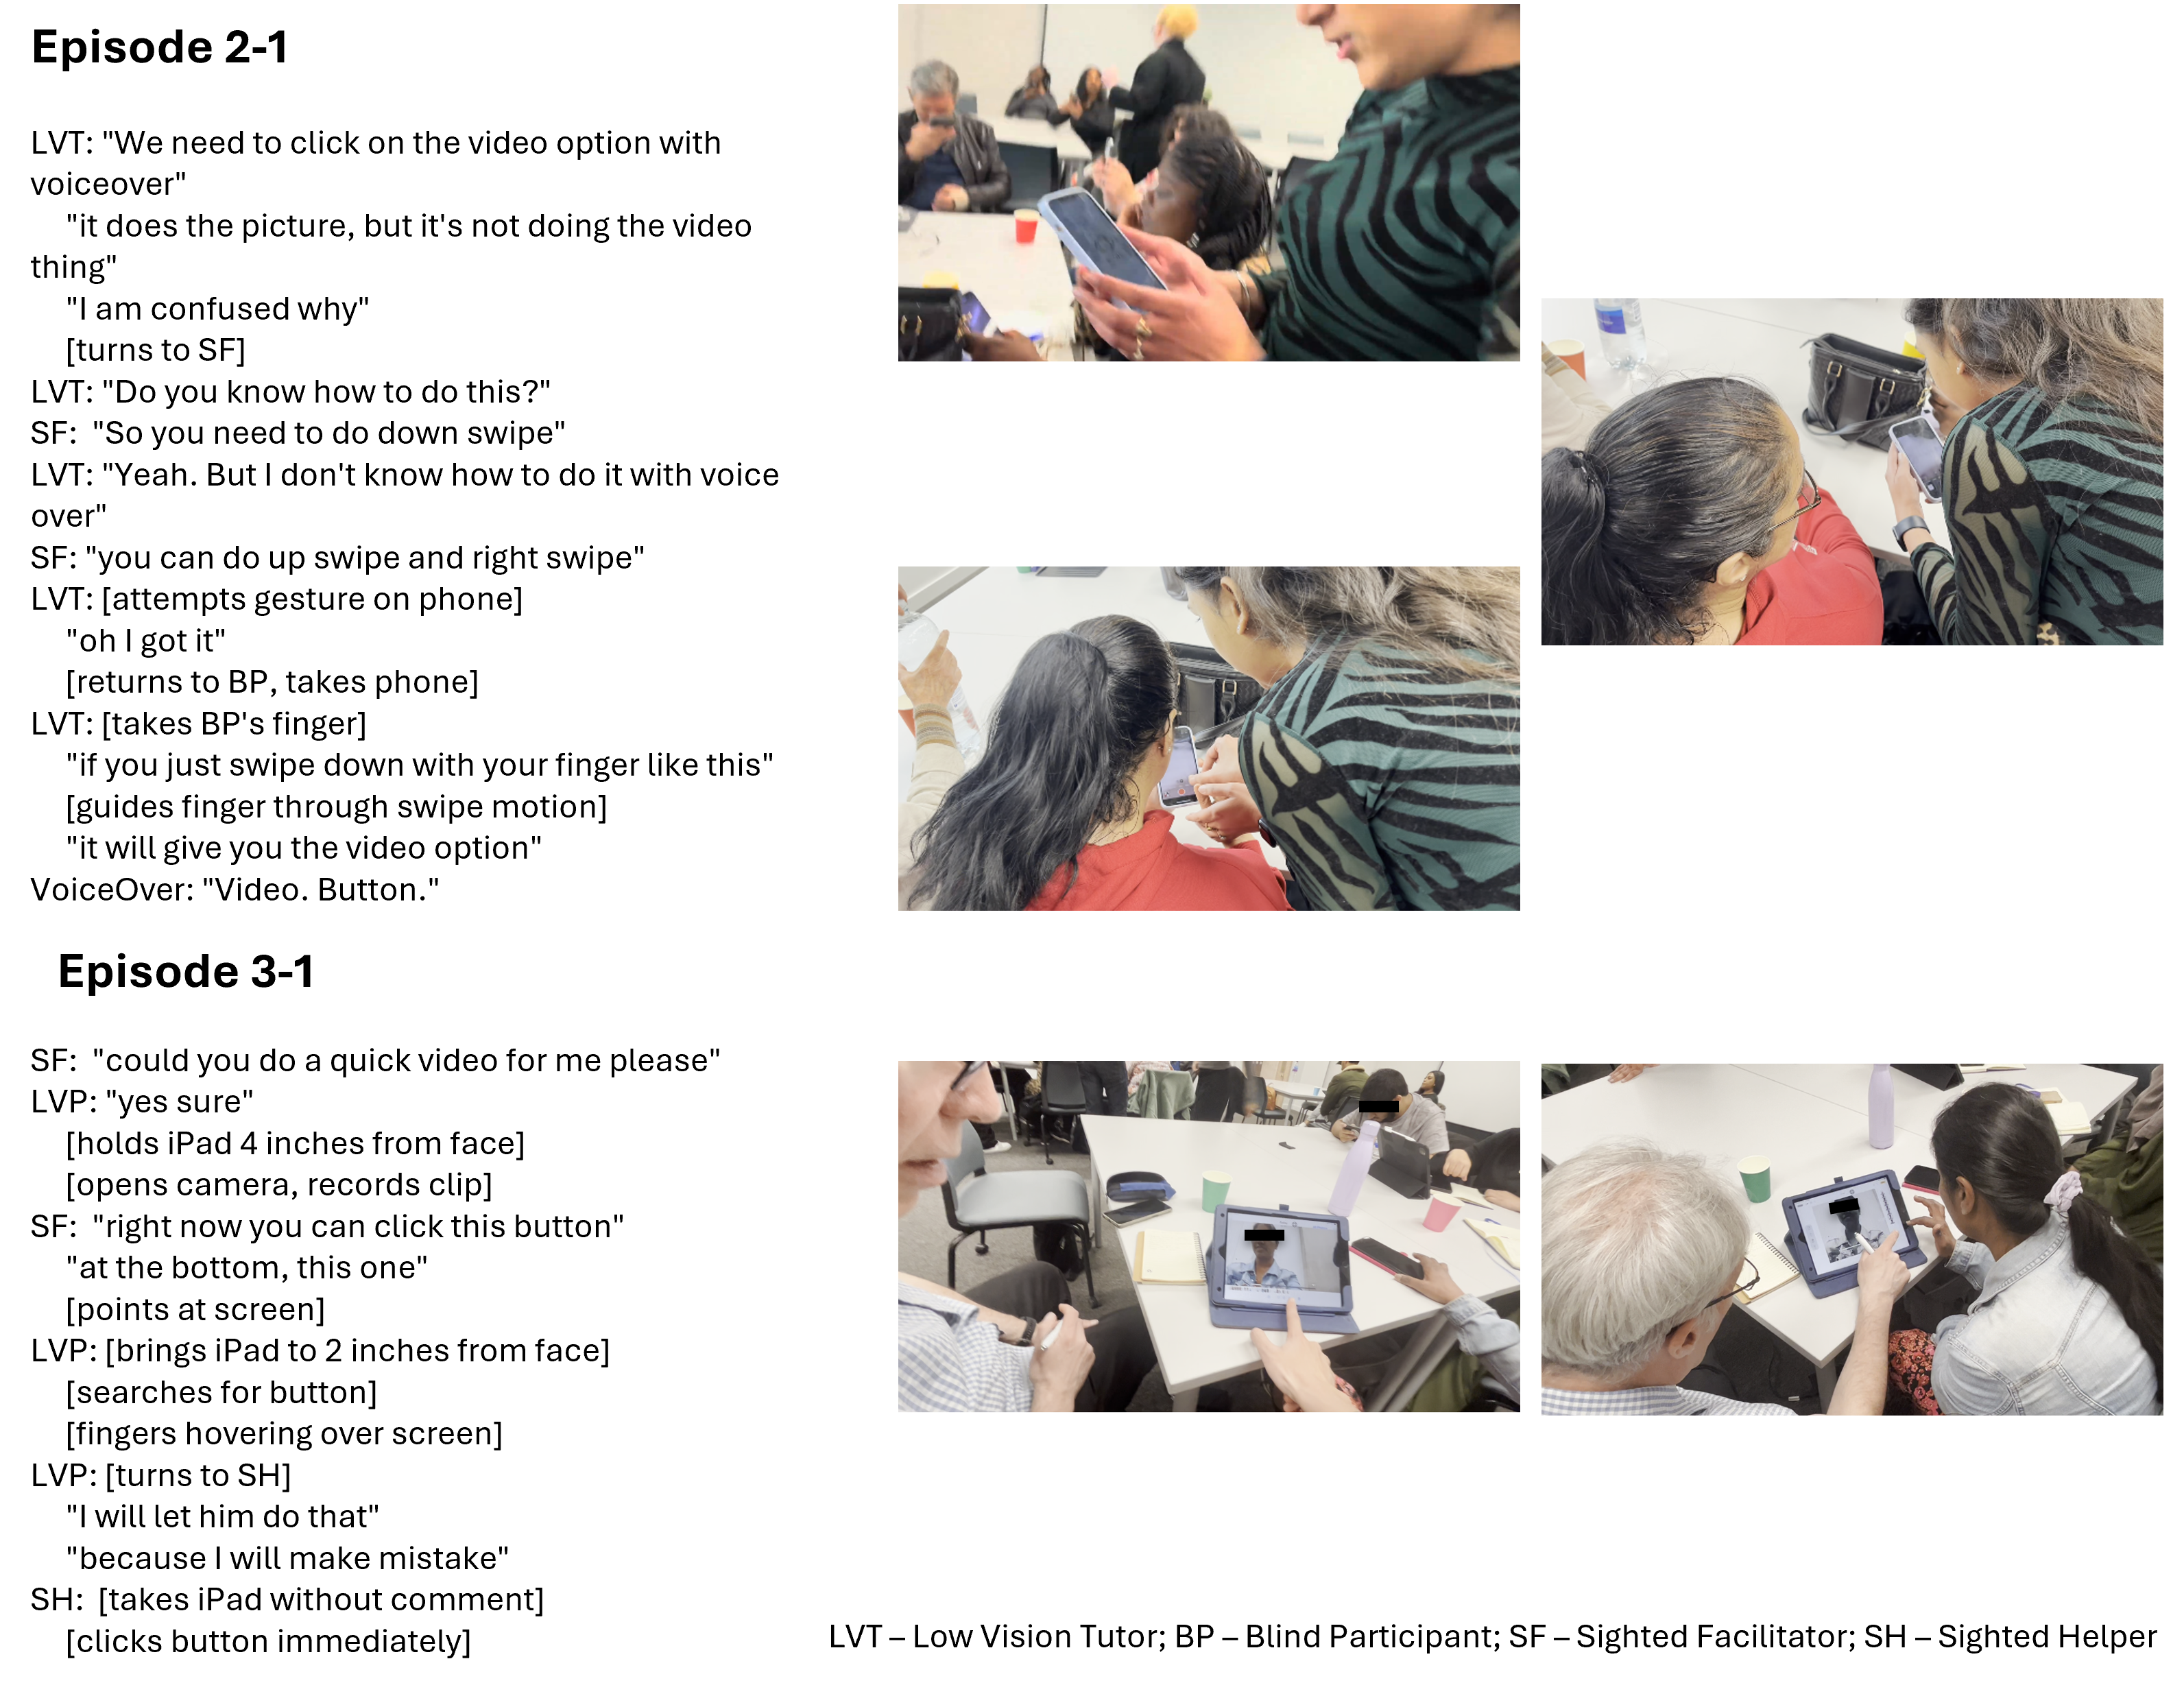
\includegraphics[width=1\linewidth]{Pics/Pattern_2.png}
     \caption{Collaborative patterns: Cross-modal translation (Episode 2-1) and task-specific delegation(Episode 3-1) }
     \label{fig:paatern2}

\Description{Five-photo collage showing collaborative exploration of mobile filming and editing. Top left: wide view of a classroom with people at tables; a facilitator checks a participant’s phone. Top right: two women review footage on a phone. Centre: a close view of a participant pointing to options on another person’s phone. Bottom left and bottom right: pairs review clips on a tablet, with one person pointing to the on-screen timeline. Images highlight peer learning, reviewing recordings, and simple edits on phones and tablets.}
 \end{figure}
\subsubsection{Pattern 2: Cross-Modal Translation}
When dyads reach their limit, they often recruit a third party. This strategy appears when helpers mark the boundary of their current knowledge and invite joint problem solving without abandoning their role. The newly added collaborator typically contributes a missing rule or gesture, which then must be translated into VoiceOver-compatible action for the blind participant.

\textbf{Episode 2-1: }In the VoiceOver mode-switch scene (\autoref{fig:paatern2}), the low-vision tutor identifies the current state (“picture” rather than “video”), then states the procedural gap: “it is not doing the video thing. I am confused why.” She then went for the sighted facilitator for help. a sighted facilitator provides the procedural key as gesture talk (“you need to do down swipe”). The low-vision tutor differentiates concept and implementation (“I do not know how to do it with VoiceOver”). After a brief, mid-air demonstration with verbal accompaniment (“you can do up swipe and right swipe”), the tutor practices and signals uptake (“oh I got it”). Only then can they relay the instruction haptically, taking the participant’s finger and guiding the on-screen motion while narrating the VoiceOver outcome (“if you swipe down, it will give you the video option”). The low-vision collaborator operates as a modality relay: sighted gestural instruction becomes embodied skill, then becomes tactile coaching aligned with the screen reader.

\subsubsection{Pattern 3: Task-Specific Delegation Protocols}
Low-vision participants actively manage independence and accuracy, switching between solo action and targeted hand-off.

\textbf{Episode 3-1: }In the iPad editing episode (\autoref{fig:paatern2}), a low-vision participant confidently records a short clip with the device 4 inches from their face. When asked to “click this button, at the bottom, this one,” the device shifts closer, to roughly 2 inches, indicating increasing visual strain for smaller, less familiar controls. Fingers hover near the region, suggesting approximate knowledge but risk of error. The participant then states, “I will let him do that because I will make mistake,” and hands the device to a sighted helper, who selects the control without negotiation. Delegation is framed as error prevention rather than inability, preserving agency while meeting the task requirement.

\subsubsection{Pattern 4: Peer-to-Peer Assistance  }
During remote workshops, participants with advanced technical skills emerge as peer coaches, providing targeted procedural guidance that bridges knowledge gaps. These peer experts demonstrate deep understanding of both the technology and the accessibility features, offering precise instructions that preserve learner agency while ensuring task completion.

\textbf{Episode 4-1: Spatial Navigation Expertise}
When participants struggle with camera mode switching, a blind participant with extensive iPhone experience, provides precise spatial guidance: "You go to the bottom right hand corner. And that is where... if you wish to change the video, you go slightly further up than the shutter. And that's where you will find the mode button" He then details the gesture mechanics: "It's a flick. You do a vertical flick, so you put your finger on it and then you do a vertical flick either up or down." This demonstrates how blind experts develop and share detailed mental maps of interface layouts, translating spatial relationships into actionable instructions. He also corrects misconceptions about navigation methods, demonstrating his deep VoiceOver expertise: "May I just say when it comes to the iPhone, there's no swiping. You go to the bottom right hand corner, you'll see, back camera or front. All you do is just double tap on it and it will change" His correction shows how peer experts understand the distinction between different navigation modes and can guide others to the most efficient interaction patterns.
